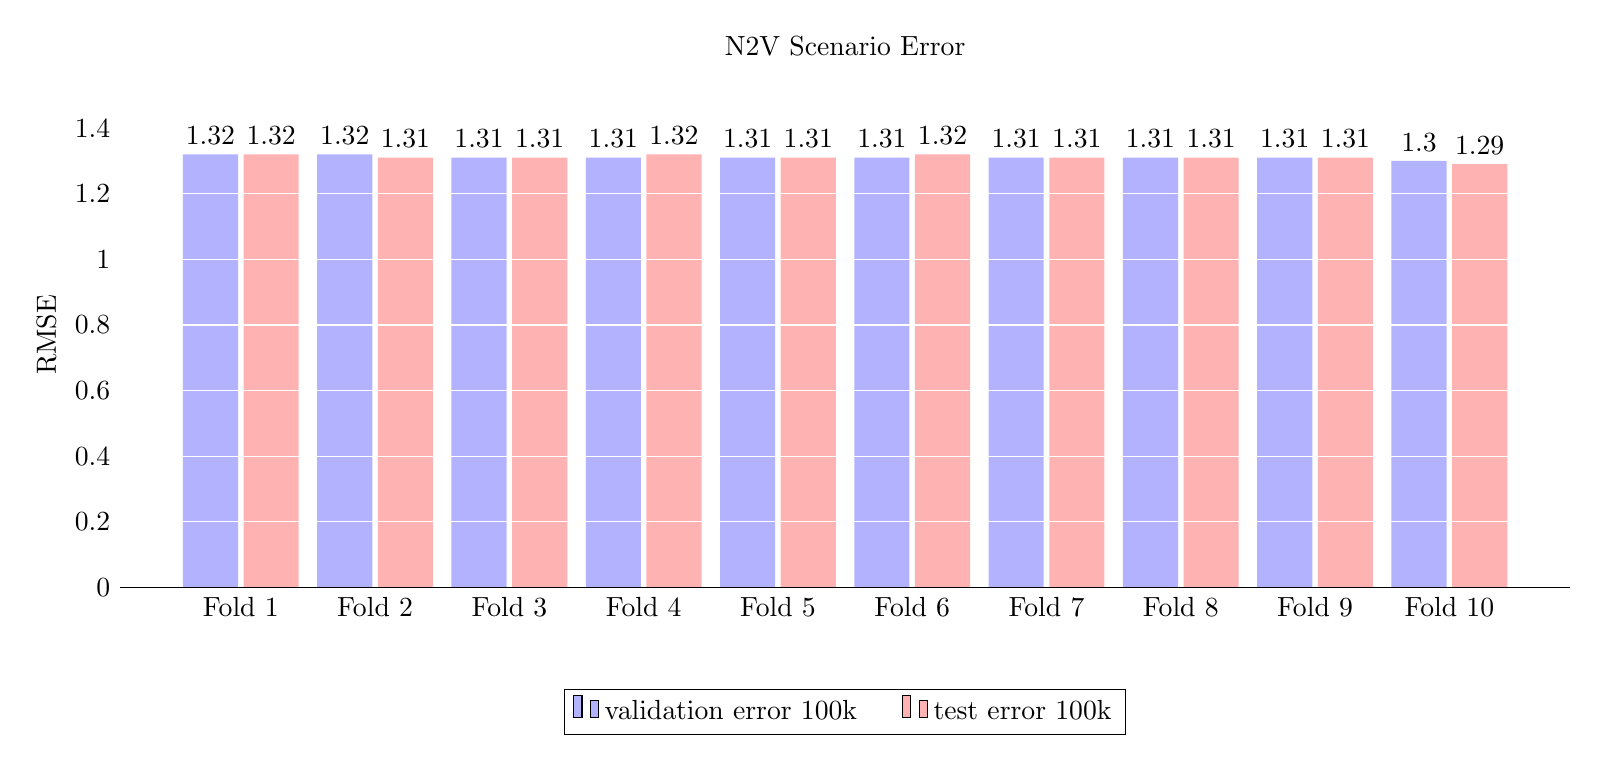
\begin{tikzpicture}
  \centering
  \begin{axis}[
        ybar, axis on top,
        title={N2V Scenario Error},
        height=8cm, width=20cm,
        bar width=0.7cm,
        ymajorgrids, tick align=inside,
        major grid style={draw=white},
        enlarge y limits={value=.1,upper},
        ymin=0, ymax=1.4,
        axis x line*=bottom,
        y axis line style={opacity=0},
        tickwidth=0pt,
        enlarge x limits=true,
        legend style={
            at={(0.5,-0.2)},
            anchor=north,
            legend columns=-1,
            /tikz/every even column/.append style={column sep=0.5cm}
        },
        ylabel={RMSE},
        symbolic x coords={
           Fold 1,Fold 2,
           Fold 3,Fold 4,
           Fold 5,Fold 6,
           Fold 7,Fold 8,
           Fold 9,Fold 10},
       xtick=data,
       nodes near coords={
        \pgfmathprintnumber[precision=2]{\pgfplotspointmeta}
       }
    ]
    \addplot [draw=none, fill=blue!30] coordinates {
      (Fold 1, 1.32)
      (Fold 2, 1.32)
      (Fold 3, 1.31)
      (Fold 4, 1.31)
      (Fold 5, 1.31)
      (Fold 6, 1.31)
      (Fold 7, 1.31)
      (Fold 8, 1.31)
      (Fold 9, 1.31)
      (Fold 10, 1.30)};
   \addplot [draw=none,fill=red!30] coordinates {
      (Fold 1, 1.32)
      (Fold 2, 1.31)
      (Fold 3, 1.31)
      (Fold 4, 1.32)
      (Fold 5, 1.31)
      (Fold 6, 1.32)
      (Fold 7, 1.31)
      (Fold 8, 1.31)
      (Fold 9, 1.31)
      (Fold 10, 1.29)};
    \legend{validation error 100k, test error 100k}
  \end{axis}
  \end{tikzpicture}